\documentclass[1p]{elsarticle_modified}
%\bibliographystyle{elsarticle-num}

%\usepackage[colorlinks]{hyperref}
%\usepackage{abbrmath_seonhwa} %\Abb, \Ascr, \Acal ,\Abf, \Afrak
\usepackage{amsfonts}
\usepackage{amssymb}
\usepackage{amsmath}
\usepackage{amsthm}
\usepackage{scalefnt}
\usepackage{amsbsy}
\usepackage{kotex}
\usepackage{caption}
\usepackage{subfig}
\usepackage{color}
\usepackage{graphicx}
\usepackage{xcolor} %% white, black, red, green, blue, cyan, magenta, yellow
\usepackage{float}
\usepackage{setspace}
\usepackage{hyperref}

\usepackage{tikz}
\usetikzlibrary{arrows}

\usepackage{multirow}
\usepackage{array} % fixed length table
\usepackage{hhline}

%%%%%%%%%%%%%%%%%%%%%
\makeatletter
\renewcommand*\env@matrix[1][\arraystretch]{%
	\edef\arraystretch{#1}%
	\hskip -\arraycolsep
	\let\@ifnextchar\new@ifnextchar
	\array{*\c@MaxMatrixCols c}}
\makeatother %https://tex.stackexchange.com/questions/14071/how-can-i-increase-the-line-spacing-in-a-matrix
%%%%%%%%%%%%%%%

\usepackage[normalem]{ulem}

\newcommand{\msout}[1]{\ifmmode\text{\sout{\ensuremath{#1}}}\else\sout{#1}\fi}
%SOURCE: \msout is \stkout macro in https://tex.stackexchange.com/questions/20609/strikeout-in-math-mode

\newcommand{\cancel}[1]{
	\ifmmode
	{\color{red}\msout{#1}}
	\else
	{\color{red}\sout{#1}}
	\fi
}

\newcommand{\add}[1]{
	{\color{blue}\uwave{#1}}
}

\newcommand{\replace}[2]{
	\ifmmode
	{\color{red}\msout{#1}}{\color{blue}\uwave{#2}}
	\else
	{\color{red}\sout{#1}}{\color{blue}\uwave{#2}}
	\fi
}

\newcommand{\Sol}{\mathcal{S}} %segment
\newcommand{\D}{D} %diagram
\newcommand{\A}{\mathcal{A}} %arc


%%%%%%%%%%%%%%%%%%%%%%%%%%%%%5 test

\def\sl{\operatorname{\textup{SL}}(2,\Cbb)}
\def\psl{\operatorname{\textup{PSL}}(2,\Cbb)}
\def\quan{\mkern 1mu \triangleright \mkern 1mu}

\theoremstyle{definition}
\newtheorem{thm}{Theorem}[section]
\newtheorem{prop}[thm]{Proposition}
\newtheorem{lem}[thm]{Lemma}
\newtheorem{ques}[thm]{Question}
\newtheorem{cor}[thm]{Corollary}
\newtheorem{defn}[thm]{Definition}
\newtheorem{exam}[thm]{Example}
\newtheorem{rmk}[thm]{Remark}
\newtheorem{alg}[thm]{Algorithm}

\newcommand{\I}{\sqrt{-1}}
\begin{document}

%\begin{frontmatter}
%
%\title{Boundary parabolic representations of knots up to 8 crossings}
%
%%% Group authors per affiliation:
%\author{Yunhi Cho} 
%\address{Department of Mathematics, University of Seoul, Seoul, Korea}
%\ead{yhcho@uos.ac.kr}
%
%
%\author{Seonhwa Kim} %\fnref{s_kim}}
%\address{Center for Geometry and Physics, Institute for Basic Science, Pohang, 37673, Korea}
%\ead{ryeona17@ibs.re.kr}
%
%\author{Hyuk Kim}
%\address{Department of Mathematical Sciences, Seoul National University, Seoul 08826, Korea}
%\ead{hyukkim@snu.ac.kr}
%
%\author{Seokbeom Yoon}
%\address{Department of Mathematical Sciences, Seoul National University, Seoul, 08826,  Korea}
%\ead{sbyoon15@snu.ac.kr}
%
%\begin{abstract}
%We find all boundary parabolic representation of knots up to 8 crossings.
%
%\end{abstract}
%\begin{keyword}
%    \MSC[2010] 57M25 
%\end{keyword}
%
%\end{frontmatter}

%\linenumbers
%\tableofcontents
%
\newcommand\colored[1]{\textcolor{white}{\rule[-0.35ex]{0.8em}{1.4ex}}\kern-0.8em\color{red} #1}%
%\newcommand\colored[1]{\textcolor{white}{ #1}\kern-2.17ex	\textcolor{white}{ #1}\kern-1.81ex	\textcolor{white}{ #1}\kern-2.15ex\color{red}#1	}

{\Large $\underline{12a_{1033}~(K12a_{1033})}$}

\setlength{\tabcolsep}{10pt}
\renewcommand{\arraystretch}{1.6}
\vspace{1cm}\begin{tabular}{m{100pt}>{\centering\arraybackslash}m{274pt}}
\multirow{5}{120pt}{
	\centering
	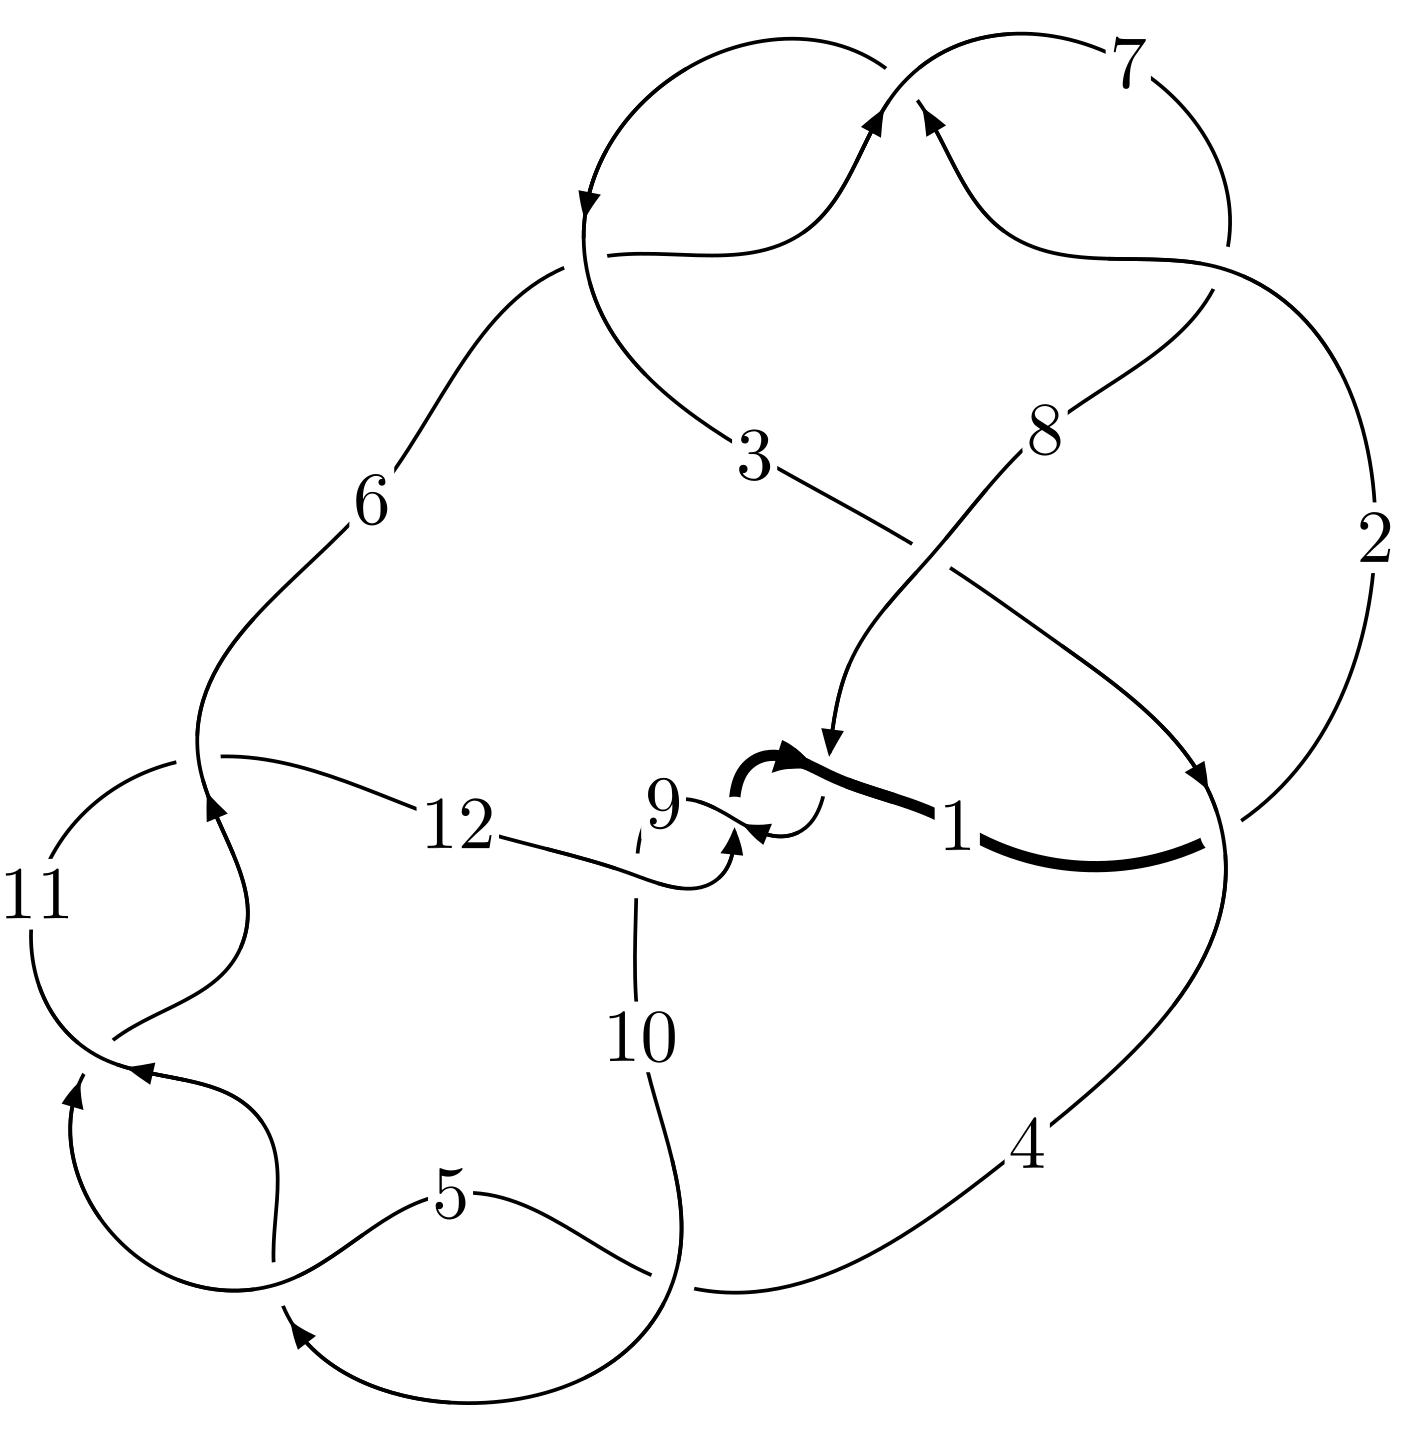
\includegraphics[width=112pt]{../../../GIT/diagram.site/Diagrams/png/1834_12a_1033.png}\\
\ \ \ A knot diagram\footnotemark}&
\allowdisplaybreaks
\textbf{Linearized knot diagam} \\
\cline{2-2}
 &
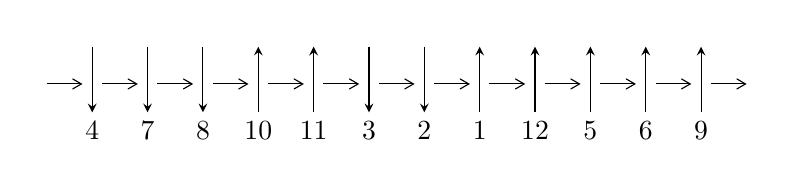
\begin{tikzpicture}[x=20pt, y=17pt]
	% nodes
	\node (C0) at (0, 0) {};
	\node (C1) at (1, 0) {};
	\node (C1U) at (1, +1) {};
	\node (C1D) at (1, -1) {4};

	\node (C2) at (2, 0) {};
	\node (C2U) at (2, +1) {};
	\node (C2D) at (2, -1) {7};

	\node (C3) at (3, 0) {};
	\node (C3U) at (3, +1) {};
	\node (C3D) at (3, -1) {8};

	\node (C4) at (4, 0) {};
	\node (C4U) at (4, +1) {};
	\node (C4D) at (4, -1) {10};

	\node (C5) at (5, 0) {};
	\node (C5U) at (5, +1) {};
	\node (C5D) at (5, -1) {11};

	\node (C6) at (6, 0) {};
	\node (C6U) at (6, +1) {};
	\node (C6D) at (6, -1) {3};

	\node (C7) at (7, 0) {};
	\node (C7U) at (7, +1) {};
	\node (C7D) at (7, -1) {2};

	\node (C8) at (8, 0) {};
	\node (C8U) at (8, +1) {};
	\node (C8D) at (8, -1) {1};

	\node (C9) at (9, 0) {};
	\node (C9U) at (9, +1) {};
	\node (C9D) at (9, -1) {12};

	\node (C10) at (10, 0) {};
	\node (C10U) at (10, +1) {};
	\node (C10D) at (10, -1) {5};

	\node (C11) at (11, 0) {};
	\node (C11U) at (11, +1) {};
	\node (C11D) at (11, -1) {6};

	\node (C12) at (12, 0) {};
	\node (C12U) at (12, +1) {};
	\node (C12D) at (12, -1) {9};
	\node (C13) at (13, 0) {};

	% arrows
	\draw[->,>={angle 60}]
	(C0) edge (C1) (C1) edge (C2) (C2) edge (C3) (C3) edge (C4) (C4) edge (C5) (C5) edge (C6) (C6) edge (C7) (C7) edge (C8) (C8) edge (C9) (C9) edge (C10) (C10) edge (C11) (C11) edge (C12) (C12) edge (C13) ;	\draw[->,>=stealth]
	(C1U) edge (C1D) (C2U) edge (C2D) (C3U) edge (C3D) (C4D) edge (C4U) (C5D) edge (C5U) (C6U) edge (C6D) (C7U) edge (C7D) (C8D) edge (C8U) (C9D) edge (C9U) (C10D) edge (C10U) (C11D) edge (C11U) (C12D) edge (C12U) ;
	\end{tikzpicture} \\
\hhline{~~} \\& 
\textbf{Solving Sequence} \\ \cline{2-2} 
 &
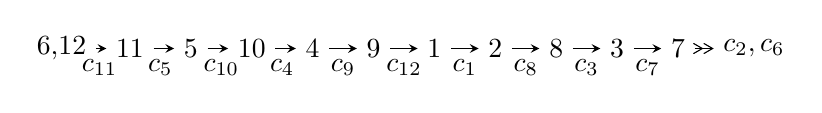
\begin{tikzpicture}[x=22pt, y=7pt]
	% node
	\node (A0) at (-1/8, 0) {6,12};
	\node (A1) at (1, 0) {11};
	\node (A2) at (2, 0) {5};
	\node (A3) at (3, 0) {10};
	\node (A4) at (4, 0) {4};
	\node (A5) at (5, 0) {9};
	\node (A6) at (6, 0) {1};
	\node (A7) at (7, 0) {2};
	\node (A8) at (8, 0) {8};
	\node (A9) at (9, 0) {3};
	\node (A10) at (10, 0) {7};
	\node (C1) at (1/2, -1) {$c_{11}$};
	\node (C2) at (3/2, -1) {$c_{5}$};
	\node (C3) at (5/2, -1) {$c_{10}$};
	\node (C4) at (7/2, -1) {$c_{4}$};
	\node (C5) at (9/2, -1) {$c_{9}$};
	\node (C6) at (11/2, -1) {$c_{12}$};
	\node (C7) at (13/2, -1) {$c_{1}$};
	\node (C8) at (15/2, -1) {$c_{8}$};
	\node (C9) at (17/2, -1) {$c_{3}$};
	\node (C10) at (19/2, -1) {$c_{7}$};
	\node (A11) at (45/4, 0) {$c_{2},c_{6}$};

	% edge
	\draw[->,>=stealth]	
	(A0) edge (A1) (A1) edge (A2) (A2) edge (A3) (A3) edge (A4) (A4) edge (A5) (A5) edge (A6) (A6) edge (A7) (A7) edge (A8) (A8) edge (A9) (A9) edge (A10) ;
	\draw[->>,>={angle 60}]	
	(A10) edge (A11);
\end{tikzpicture} \\ 

\end{tabular} \\

\footnotetext{
The image of knot diagram is generated by the software ``\textbf{Draw programme}" developed by Andrew Bartholomew(\url{http://www.layer8.co.uk/maths/draw/index.htm\#Running-draw}), where we modified some parts for our purpose(\url{https://github.com/CATsTAILs/LinksPainter}).
}\phantom \\ \newline 
\centering \textbf{Ideals for irreducible components\footnotemark of $X_{\text{par}}$} 
 
\begin{align*}
I^u_{1}&=\langle 
u^{53}- u^{52}+\cdots+u-1\rangle \\
\\
\end{align*}
\raggedright * 1 irreducible components of $\dim_{\mathbb{C}}=0$, with total 53 representations.\\
\footnotetext{All coefficients of polynomials are rational numbers. But the coefficients are sometimes approximated in decimal forms when there is not enough margin.}
\newpage
\renewcommand{\arraystretch}{1}
\centering \section*{I. $I^u_{1}= \langle u^{53}- u^{52}+\cdots+u-1 \rangle$}
\flushleft \textbf{(i) Arc colorings}\\
\begin{tabular}{m{7pt} m{180pt} m{7pt} m{180pt} }
\flushright $a_{6}=$&$\begin{pmatrix}0\\u\end{pmatrix}$ \\
\flushright $a_{12}=$&$\begin{pmatrix}1\\0\end{pmatrix}$ \\
\flushright $a_{11}=$&$\begin{pmatrix}1\\u^2\end{pmatrix}$ \\
\flushright $a_{5}=$&$\begin{pmatrix}- u\\- u^3+u\end{pmatrix}$ \\
\flushright $a_{10}=$&$\begin{pmatrix}- u^2+1\\- u^4+2 u^2\end{pmatrix}$ \\
\flushright $a_{4}=$&$\begin{pmatrix}u^3-2 u\\u^5-3 u^3+u\end{pmatrix}$ \\
\flushright $a_{9}=$&$\begin{pmatrix}u^4-3 u^2+1\\- u^4+2 u^2\end{pmatrix}$ \\
\flushright $a_{1}=$&$\begin{pmatrix}u^8-5 u^6+7 u^4-2 u^2+1\\- u^8+4 u^6-4 u^4\end{pmatrix}$ \\
\flushright $a_{2}=$&$\begin{pmatrix}u^{16}-9 u^{14}+31 u^{12}-50 u^{10}+39 u^8-22 u^6+18 u^4-4 u^2+1\\u^{18}-10 u^{16}+39 u^{14}-74 u^{12}+71 u^{10}-40 u^8+26 u^6-12 u^4+u^2\end{pmatrix}$ \\
\flushright $a_{8}=$&$\begin{pmatrix}u^{12}-7 u^{10}+17 u^8-16 u^6+6 u^4-5 u^2+1\\- u^{12}+6 u^{10}-12 u^8+8 u^6- u^4+2 u^2\end{pmatrix}$ \\
\flushright $a_{3}=$&$\begin{pmatrix}u^{29}-16 u^{27}+\cdots-8 u^3- u\\- u^{29}+15 u^{27}+\cdots- u^3+u\end{pmatrix}$ \\
\flushright $a_{7}=$&$\begin{pmatrix}- u^{46}+25 u^{44}+\cdots-4 u^2+1\\- u^{48}+26 u^{46}+\cdots+4 u^6+2 u^2\end{pmatrix}$\\&\end{tabular}
\flushleft \textbf{(ii) Obstruction class $= -1$}\\~\\
\flushleft \textbf{(iii) Cusp Shapes $= -4 u^{50}+108 u^{48}+\cdots+4 u+6$}\\~\\
\newpage\renewcommand{\arraystretch}{1}
\flushleft \textbf{(iv) u-Polynomials at the component}\newline \\
\begin{tabular}{m{50pt}|m{274pt}}
Crossings & \hspace{64pt}u-Polynomials at each crossing \\
\hline $$\begin{aligned}c_{1}\end{aligned}$$&$\begin{aligned}
&u^{53}-13 u^{52}+\cdots-51 u+3
\end{aligned}$\\
\hline $$\begin{aligned}c_{2},c_{6},c_{7}\end{aligned}$$&$\begin{aligned}
&u^{53}+u^{52}+\cdots- u-1
\end{aligned}$\\
\hline $$\begin{aligned}c_{3}\end{aligned}$$&$\begin{aligned}
&u^{53}- u^{52}+\cdots-3 u-5
\end{aligned}$\\
\hline $$\begin{aligned}c_{4},c_{5},c_{10}\\c_{11}\end{aligned}$$&$\begin{aligned}
&u^{53}- u^{52}+\cdots+u-1
\end{aligned}$\\
\hline $$\begin{aligned}c_{8},c_{9},c_{12}\end{aligned}$$&$\begin{aligned}
&u^{53}+7 u^{52}+\cdots+81 u+7
\end{aligned}$\\
\hline
\end{tabular}\\~\\
\newpage\renewcommand{\arraystretch}{1}
\flushleft \textbf{(v) Riley Polynomials at the component}\newline \\
\begin{tabular}{m{50pt}|m{274pt}}
Crossings & \hspace{64pt}Riley Polynomials at each crossing \\
\hline $$\begin{aligned}c_{1}\end{aligned}$$&$\begin{aligned}
&y^{53}+3 y^{52}+\cdots-393 y-9
\end{aligned}$\\
\hline $$\begin{aligned}c_{2},c_{6},c_{7}\end{aligned}$$&$\begin{aligned}
&y^{53}+47 y^{52}+\cdots+3 y-1
\end{aligned}$\\
\hline $$\begin{aligned}c_{3}\end{aligned}$$&$\begin{aligned}
&y^{53}-5 y^{52}+\cdots-221 y-25
\end{aligned}$\\
\hline $$\begin{aligned}c_{4},c_{5},c_{10}\\c_{11}\end{aligned}$$&$\begin{aligned}
&y^{53}-57 y^{52}+\cdots+3 y-1
\end{aligned}$\\
\hline $$\begin{aligned}c_{8},c_{9},c_{12}\end{aligned}$$&$\begin{aligned}
&y^{53}+51 y^{52}+\cdots+247 y-49
\end{aligned}$\\
\hline
\end{tabular}\\~\\
\newpage\flushleft \textbf{(vi) Complex Volumes and Cusp Shapes}
$$\begin{array}{c|c|c}  
\text{Solutions to }I^u_{1}& \I (\text{vol} + \sqrt{-1}CS) & \text{Cusp shape}\\
 \hline 
\begin{aligned}
u &= -0.548575 + 0.633673 I\end{aligned}
 & -1.51521 - 10.00010 I & \phantom{-}2.58535 + 7.98539 I \\ \hline\begin{aligned}
u &= -0.548575 - 0.633673 I\end{aligned}
 & -1.51521 + 10.00010 I & \phantom{-}2.58535 - 7.98539 I \\ \hline\begin{aligned}
u &= \phantom{-}0.535266 + 0.635034 I\end{aligned}
 & -6.68651 + 6.22464 I & -2.12914 - 7.04200 I \\ \hline\begin{aligned}
u &= \phantom{-}0.535266 - 0.635034 I\end{aligned}
 & -6.68651 - 6.22464 I & -2.12914 + 7.04200 I \\ \hline\begin{aligned}
u &= -0.512310 + 0.631969 I\end{aligned}
 & -4.69465 - 2.29803 I & \phantom{-}0.49220 + 2.27561 I \\ \hline\begin{aligned}
u &= -0.512310 - 0.631969 I\end{aligned}
 & -4.69465 + 2.29803 I & \phantom{-}0.49220 - 2.27561 I \\ \hline\begin{aligned}
u &= -0.487905 + 0.637564 I\end{aligned}
 & -4.76749 - 1.99907 I & \phantom{-}0.17746 + 4.07491 I \\ \hline\begin{aligned}
u &= -0.487905 - 0.637564 I\end{aligned}
 & -4.76749 + 1.99907 I & \phantom{-}0.17746 - 4.07491 I \\ \hline\begin{aligned}
u &= \phantom{-}0.464669 + 0.647606 I\end{aligned}
 & -6.89567 - 1.88935 I & -2.89485 + 0.79576 I \\ \hline\begin{aligned}
u &= \phantom{-}0.464669 - 0.647606 I\end{aligned}
 & -6.89567 + 1.88935 I & -2.89485 - 0.79576 I \\ \hline\begin{aligned}
u &= -0.449493 + 0.651810 I\end{aligned}
 & -1.80864 + 5.65716 I & \phantom{-}1.70059 - 1.94125 I \\ \hline\begin{aligned}
u &= -0.449493 - 0.651810 I\end{aligned}
 & -1.80864 - 5.65716 I & \phantom{-}1.70059 + 1.94125 I \\ \hline\begin{aligned}
u &= \phantom{-}0.504505 + 0.567177 I\end{aligned}
 & \phantom{-}1.97412 + 1.94133 I & \phantom{-}4.71944 - 3.76784 I \\ \hline\begin{aligned}
u &= \phantom{-}0.504505 - 0.567177 I\end{aligned}
 & \phantom{-}1.97412 - 1.94133 I & \phantom{-}4.71944 + 3.76784 I \\ \hline\begin{aligned}
u &= \phantom{-}0.652033 + 0.329464 I\end{aligned}
 & \phantom{-}5.34002 + 6.28128 I & \phantom{-}8.12896 - 8.54610 I \\ \hline\begin{aligned}
u &= \phantom{-}0.652033 - 0.329464 I\end{aligned}
 & \phantom{-}5.34002 - 6.28128 I & \phantom{-}8.12896 + 8.54610 I \\ \hline\begin{aligned}
u &= -0.687986 + 0.156912 I\end{aligned}
 & \phantom{-}6.28732 + 1.58298 I & \phantom{-}11.28727 + 0.73154 I \\ \hline\begin{aligned}
u &= -0.687986 - 0.156912 I\end{aligned}
 & \phantom{-}6.28732 - 1.58298 I & \phantom{-}11.28727 - 0.73154 I \\ \hline\begin{aligned}
u &= -0.591945 + 0.318276 I\end{aligned}
 & \phantom{-}0.12349 - 3.23267 I & \phantom{-}3.04126 + 9.49675 I \\ \hline\begin{aligned}
u &= -0.591945 - 0.318276 I\end{aligned}
 & \phantom{-}0.12349 + 3.23267 I & \phantom{-}3.04126 - 9.49675 I \\ \hline\begin{aligned}
u &= \phantom{-}0.372482 + 0.439549 I\end{aligned}
 & \phantom{-}1.98957 + 1.52097 I & \phantom{-}1.80190 - 4.43655 I \\ \hline\begin{aligned}
u &= \phantom{-}0.372482 - 0.439549 I\end{aligned}
 & \phantom{-}1.98957 - 1.52097 I & \phantom{-}1.80190 + 4.43655 I \\ \hline\begin{aligned}
u &= \phantom{-}0.541460 + 0.168929 I\end{aligned}
 & \phantom{-}1.006470 + 0.410735 I & \phantom{-}8.40701 - 1.41779 I \\ \hline\begin{aligned}
u &= \phantom{-}0.541460 - 0.168929 I\end{aligned}
 & \phantom{-}1.006470 - 0.410735 I & \phantom{-}8.40701 + 1.41779 I \\ \hline\begin{aligned}
u &= \phantom{-}1.45482\phantom{ +0.000000I}\end{aligned}
 & \phantom{-}3.97144\phantom{ +0.000000I} & \phantom{-0.000000 } 0 \\ \hline\begin{aligned}
u &= -1.45391 + 0.05193 I\end{aligned}
 & \phantom{-}7.75885 - 3.05240 I & \phantom{-0.000000 } 0 \\ \hline\begin{aligned}
u &= -1.45391 - 0.05193 I\end{aligned}
 & \phantom{-}7.75885 + 3.05240 I & \phantom{-0.000000 } 0 \\ \hline\begin{aligned}
u &= \phantom{-}1.47881 + 0.19165 I\end{aligned}
 & \phantom{-}4.44453 - 2.64829 I & \phantom{-0.000000 } 0 \\ \hline\begin{aligned}
u &= \phantom{-}1.47881 - 0.19165 I\end{aligned}
 & \phantom{-}4.44453 + 2.64829 I & \phantom{-0.000000 } 0 \\ \hline\begin{aligned}
u &= -1.49019 + 0.19296 I\end{aligned}
 & -0.532397 - 1.115270 I & \phantom{-0.000000 } 0\\
 \hline 
 \end{array}$$\newpage$$\begin{array}{c|c|c}  
\text{Solutions to }I^u_{1}& \I (\text{vol} + \sqrt{-1}CS) & \text{Cusp shape}\\
 \hline 
\begin{aligned}
u &= -1.49019 - 0.19296 I\end{aligned}
 & -0.532397 + 1.115270 I & \phantom{-0.000000 } 0 \\ \hline\begin{aligned}
u &= \phantom{-}1.50599 + 0.19300 I\end{aligned}
 & \phantom{-}1.75894 + 4.97978 I & \phantom{-0.000000 } 0 \\ \hline\begin{aligned}
u &= \phantom{-}1.50599 - 0.19300 I\end{aligned}
 & \phantom{-}1.75894 - 4.97978 I & \phantom{-0.000000 } 0 \\ \hline\begin{aligned}
u &= \phantom{-}0.107192 + 0.466806 I\end{aligned}
 & \phantom{-}3.69238 - 3.52663 I & \phantom{-}1.88659 + 2.63338 I \\ \hline\begin{aligned}
u &= \phantom{-}0.107192 - 0.466806 I\end{aligned}
 & \phantom{-}3.69238 + 3.52663 I & \phantom{-}1.88659 - 2.63338 I \\ \hline\begin{aligned}
u &= \phantom{-}1.52075 + 0.19227 I\end{aligned}
 & \phantom{-}1.99021 + 5.26775 I & \phantom{-0.000000 } 0 \\ \hline\begin{aligned}
u &= \phantom{-}1.52075 - 0.19227 I\end{aligned}
 & \phantom{-}1.99021 - 5.26775 I & \phantom{-0.000000 } 0 \\ \hline\begin{aligned}
u &= -1.52792 + 0.16778 I\end{aligned}
 & \phantom{-}8.71759 - 4.57599 I & \phantom{-0.000000 } 0 \\ \hline\begin{aligned}
u &= -1.52792 - 0.16778 I\end{aligned}
 & \phantom{-}8.71759 + 4.57599 I & \phantom{-0.000000 } 0 \\ \hline\begin{aligned}
u &= -1.54203 + 0.04830 I\end{aligned}
 & \phantom{-}8.05739 - 1.20567 I & \phantom{-0.000000 } 0 \\ \hline\begin{aligned}
u &= -1.54203 - 0.04830 I\end{aligned}
 & \phantom{-}8.05739 + 1.20567 I & \phantom{-0.000000 } 0 \\ \hline\begin{aligned}
u &= -1.53145 + 0.19702 I\end{aligned}
 & \phantom{-}0.12630 - 9.24228 I & \phantom{-0.000000 } 0 \\ \hline\begin{aligned}
u &= -1.53145 - 0.19702 I\end{aligned}
 & \phantom{-}0.12630 + 9.24228 I & \phantom{-0.000000 } 0 \\ \hline\begin{aligned}
u &= \phantom{-}1.53796 + 0.19740 I\end{aligned}
 & \phantom{-}5.37483 + 13.02300 I & \phantom{-0.000000 } 0 \\ \hline\begin{aligned}
u &= \phantom{-}1.53796 - 0.19740 I\end{aligned}
 & \phantom{-}5.37483 - 13.02300 I & \phantom{-0.000000 } 0 \\ \hline\begin{aligned}
u &= \phantom{-}1.54965 + 0.07623 I\end{aligned}
 & \phantom{-}7.32443 + 4.59016 I & \phantom{-0.000000 } 0 \\ \hline\begin{aligned}
u &= \phantom{-}1.54965 - 0.07623 I\end{aligned}
 & \phantom{-}7.32443 - 4.59016 I & \phantom{-0.000000 } 0 \\ \hline\begin{aligned}
u &= -1.56535 + 0.08054 I\end{aligned}
 & \phantom{-}12.8092 - 7.7128 I & \phantom{-0.000000 } 0 \\ \hline\begin{aligned}
u &= -1.56535 - 0.08054 I\end{aligned}
 & \phantom{-}12.8092 + 7.7128 I & \phantom{-0.000000 } 0 \\ \hline\begin{aligned}
u &= \phantom{-}1.56726 + 0.03872 I\end{aligned}
 & \phantom{-}13.86820 - 0.89997 I & \phantom{-0.000000 } 0 \\ \hline\begin{aligned}
u &= \phantom{-}1.56726 - 0.03872 I\end{aligned}
 & \phantom{-}13.86820 + 0.89997 I & \phantom{-0.000000 } 0 \\ \hline\begin{aligned}
u &= -0.176376 + 0.389345 I\end{aligned}
 & -1.109150 + 0.706645 I & -4.66602 - 1.44909 I \\ \hline\begin{aligned}
u &= -0.176376 - 0.389345 I\end{aligned}
 & -1.109150 - 0.706645 I & -4.66602 + 1.44909 I\\
 \hline 
 \end{array}$$\newpage
\newpage\renewcommand{\arraystretch}{1}
\centering \section*{ II. u-Polynomials}
\begin{tabular}{m{50pt}|m{274pt}}
Crossings & \hspace{64pt}u-Polynomials at each crossing \\
\hline $$\begin{aligned}c_{1}\end{aligned}$$&$\begin{aligned}
&u^{53}-13 u^{52}+\cdots-51 u+3
\end{aligned}$\\
\hline $$\begin{aligned}c_{2},c_{6},c_{7}\end{aligned}$$&$\begin{aligned}
&u^{53}+u^{52}+\cdots- u-1
\end{aligned}$\\
\hline $$\begin{aligned}c_{3}\end{aligned}$$&$\begin{aligned}
&u^{53}- u^{52}+\cdots-3 u-5
\end{aligned}$\\
\hline $$\begin{aligned}c_{4},c_{5},c_{10}\\c_{11}\end{aligned}$$&$\begin{aligned}
&u^{53}- u^{52}+\cdots+u-1
\end{aligned}$\\
\hline $$\begin{aligned}c_{8},c_{9},c_{12}\end{aligned}$$&$\begin{aligned}
&u^{53}+7 u^{52}+\cdots+81 u+7
\end{aligned}$\\
\hline
\end{tabular}\newpage\renewcommand{\arraystretch}{1}
\centering \section*{ III. Riley Polynomials}
\begin{tabular}{m{50pt}|m{274pt}}
Crossings & \hspace{64pt}Riley Polynomials at each crossing \\
\hline $$\begin{aligned}c_{1}\end{aligned}$$&$\begin{aligned}
&y^{53}+3 y^{52}+\cdots-393 y-9
\end{aligned}$\\
\hline $$\begin{aligned}c_{2},c_{6},c_{7}\end{aligned}$$&$\begin{aligned}
&y^{53}+47 y^{52}+\cdots+3 y-1
\end{aligned}$\\
\hline $$\begin{aligned}c_{3}\end{aligned}$$&$\begin{aligned}
&y^{53}-5 y^{52}+\cdots-221 y-25
\end{aligned}$\\
\hline $$\begin{aligned}c_{4},c_{5},c_{10}\\c_{11}\end{aligned}$$&$\begin{aligned}
&y^{53}-57 y^{52}+\cdots+3 y-1
\end{aligned}$\\
\hline $$\begin{aligned}c_{8},c_{9},c_{12}\end{aligned}$$&$\begin{aligned}
&y^{53}+51 y^{52}+\cdots+247 y-49
\end{aligned}$\\
\hline
\end{tabular}
\vskip 2pc
\end{document}